\documentclass[final]{beamer} 
\mode<presentation> {
  \usetheme{Berlin}
}

\usepackage{url}
\usepackage[utf8]{inputenc}
\usepackage{amsmath,amsthm, amssymb, latexsym}
\usefonttheme[onlymath]{serif}
\boldmath
\usepackage[size=custom,width=90,height=150,scale=2,orientation=landscape]{beamerposter}
\title{Guampa Poster}
\author{HLTDI}
\institute[Indiana University]{School of Informatics and Computing, Indiana University}
\date{May 29, 2014}
\begin{document}

\begin{frame}{} 
  \begin{block}
    {\centering \Huge Guampa: a Toolkit for Collaborative Translation}\par
    \centering
    {\large Alex Rudnick, Taylor Skidmore, Alberto Samaniego, and Michael Gasser}
    \par
  \end{block}

\begin{columns}[t]

%%% left column %%% 
  \begin{column}{.32\linewidth}

  \vfill
  %%\begin{block}{\large Contributions}
  \begin{block}{\large Guampa: Online Collaborative Translation}
    \centering
    \begin{itemize}
    \item Work together to translate documents
    \item Discuss translations to help others learn
    \item For building resources for under-served languages
    \item Also helps NLP researchers build bigger corpora for MT system training
    \item Designed in cooperation with educators in Paraguay for online and
    classroom use
    \end{itemize}
  \end{block}

  \begin{block}{\large Guampa Features}
    \centering
    \begin{itemize}
    \item Automatic import of Wikipedia documents and export of translated texts
    \item Integrated dictionaries to help learners
    \item Interface designed for online reading
    \item Upload and tag documents to be translated
    \item Easy login with \emph{Persona} from Mozilla
    \item Language-independent design, easy to set up and localize for your
    favorite language pair. Currently in Spanish and English.
    \item Features for supporting classes coming soon!
    \end{itemize}
  \end{block}
  \centering

  \centering
  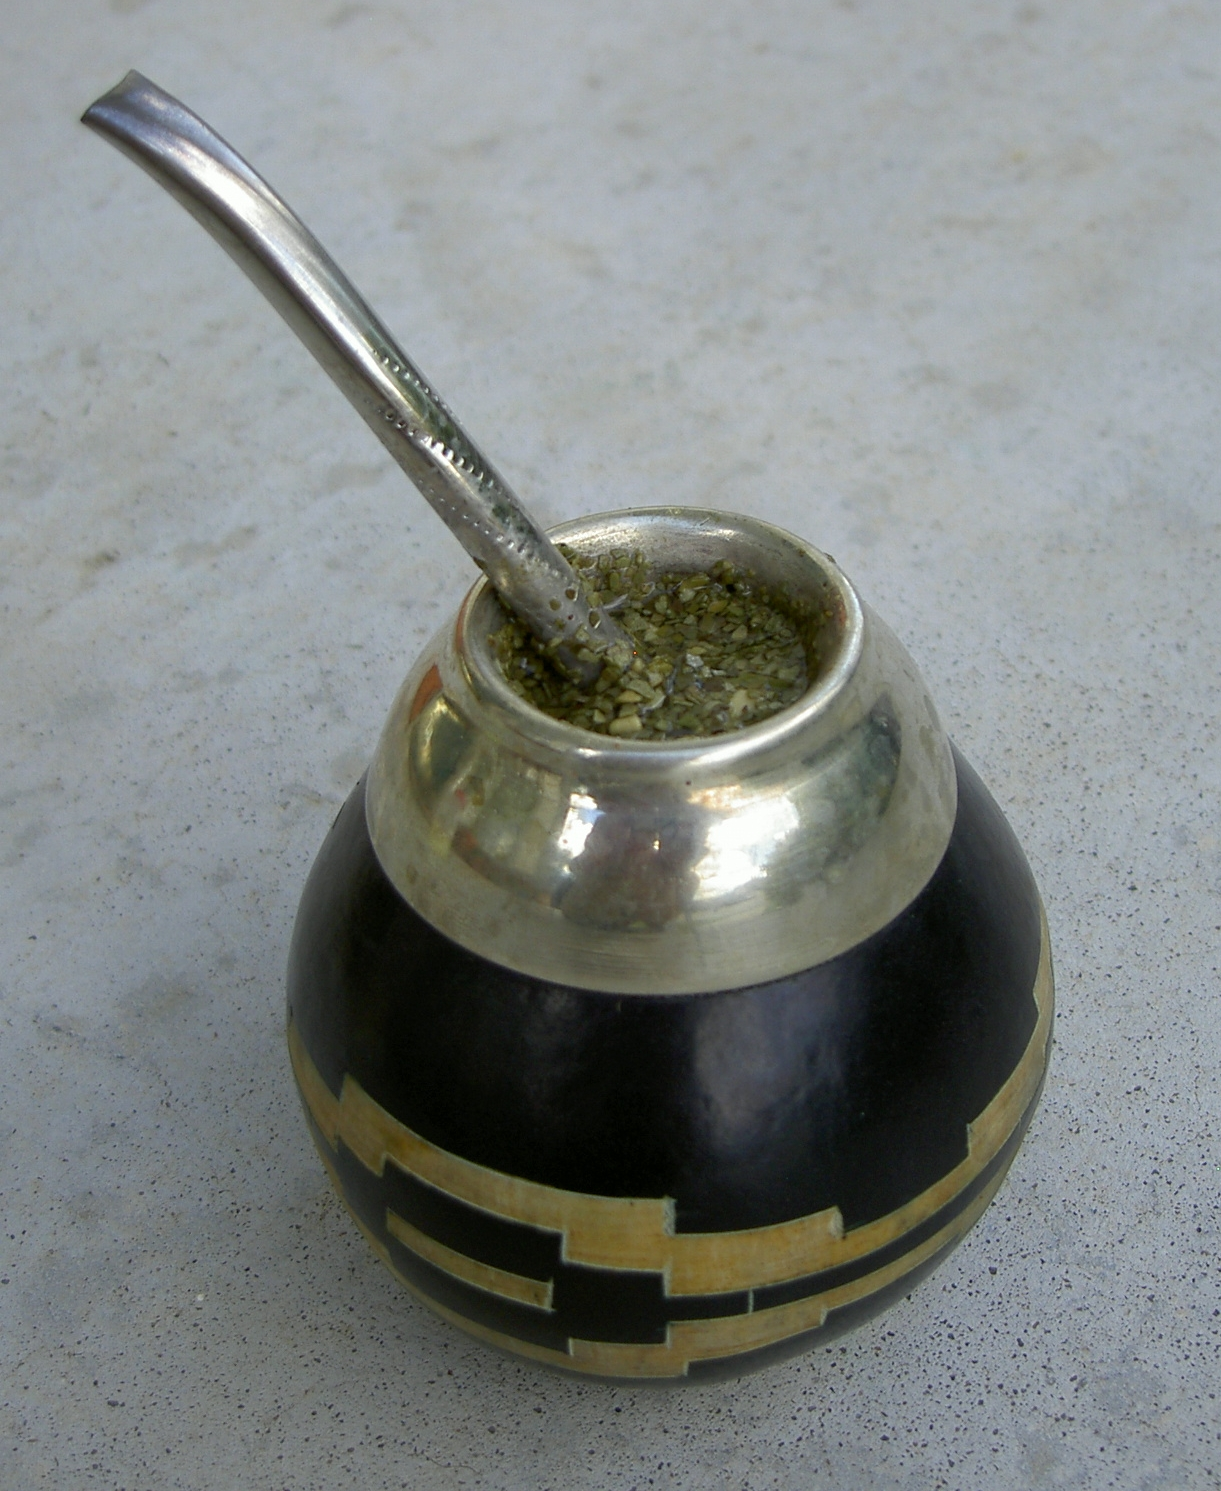
\includegraphics[width=.3\linewidth]{guampa_mate.jpg}
  \end{column}

  %%% middle column %%%
  \begin{column}{.32\linewidth}
  \vfill
  \begin{block}{\large Under-Resourced Languages}
    \begin{itemize}
    \item Roughly 7000 languages in the world -- how many do you speak?
    \item We want to support translation into languages with many speakers
    but not lots of data.
    \item Focusing on Paraguayan Guarani and Cuzco Quechua -- millions of
    speakers
    \end{itemize}
  \end{block}

  \definecolor{htmlgreen}{HTML}{008000}
  \centering
  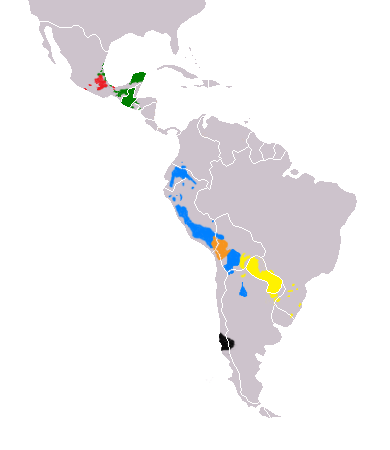
\includegraphics[width=.50\linewidth]{Map-Most_Widely_Spoken_Native_Languages_in_Latin_America.png}
  \begin{block}{\large Indigenous Languages of Latin America}
    \begin{tabular}{ll}
      {\color{blue}        $\blacksquare$} Quechua &
      {\color{yellow}      $\blacksquare$} Guarani \\
      {\color{orange}      $\blacksquare$} Aymara &
      {\color{red}         $\blacksquare$} Nahuatl \\
      {\color{htmlgreen}   $\blacksquare$} Mayan languages &
      {\color{black}       $\blacksquare$} Mapudungún \\
    \end{tabular}
  \end{block}

  \begin{block}{\large Open Source and Collaboration}
    \centering
    \begin{itemize}
    \item Working with educators in Paraguay
    \item Check out our software!
    \item \url{http://hltdi.github.io}
    \end{itemize}
  \end{block}


  \end{column}

  %%% right column %%%
  \begin{column}{.32\linewidth}
  \vfill
  \begin{block}{\large More Features}
    \begin{itemize}
    \item Frame picking the right word during translation as a word-sense disambiguation problem
    \item Languages make different distinctions!
    \item Have to learn to distinguish between uses of a source-language word
    that get translated to different target-language words
    \end{itemize}
  \end{block}

  \hfill
  \begin{center}
  
\includegraphics[width=.30\linewidth]{hltdi-logo-small.png}
  \end{center}

  \end{column}
\end{columns}
\end{frame}
\end{document}
